\chapter{Opis projektnog zadatka}
		
		\section{Motivacija i cilj}
		Cilj ovog projekta je stvoriti aplikaciju koja može na jednostavan i brz način spojiti građane i udruge za životinje kako bi se organizirale šetnje nezbrinutih pasa.\\
		Naime, broj nezbrinutih životinja raste u Hrvatskoj te je procijenjeno da ima 10 000 napuštenih životinja. Skloništa i udruge za nezbrinute životinje spašavaju ranjene i
		nezbrinute životinje, te žele potaknuti građane na angažiranost, pomoć pri brizi za
		životinje i za njihove udomljavanje. Šetnja je psima primarna potreba, a skloništa nemaju dovoljno resursa za hranu, a kamoli za plaćanje šetnji. Pretpostavljamo da bi se ljudi rado uključili u šetanje pasa kad bi postojao način, pogotovo ako planiraju usvojiti jednoga. Naša aplikacija im to odsad može i omogućiti.\\
		
		\section{Postojeća slična rješenja}
		Što se tiče postojećih rješenja iste tematike, ne postoji previše sličnosti s našim projektom. Postoje 3 web-stranice koje mogu spojiti šetače s vlasnicima pasa, no vlasnici plaćaju za te usluge te udruge nisu uključene. Prve dvije funkcioniraju na temelju oglasa - korisnik stavi oglas sa slikom svog kućnog ljubimca, vrijeme kad mu je potrebna usluga te koliko će platiti. Te stranice su:
		\begin{description}
		\item [Njuškalo:] -- najveći online oglasnik u Hrvatskoj  
		\item [Čuvalica:] -- Nacionalni portal za brigu o obitelji -- briga za djecu, starije, ljubimce 
		\end{description}
		
		Također, postoji web-stranica obrta \textbf{PETS STEP} koji nudi uslugu čuvanja i šetnje pasa. Na stranici imaju kontakt i cjenik.\par
		Kao što možemo vidjeti, u Hrvatskoj ne postoji usluga slična našoj, no u svijetu ih možemo pronaći. Najsličniji primjer bi bila web platforma \textbf{Walkzee} -- \textit{``1st free online platform connecting shelter dogs in need of a walk to dog lovers looking for a walking buddy!´´} Walkzee su stvorili Cristina i Charlie Saunders 2015. te je ideja identična kao ideja iza našeg projekta. Nažalost, njihova stranica nije zaživjela te nema mnogo udruga niti pasa na stranici. Naime, ima samo 10 stranica te 14 pasa. Osim toga, stranica izgleda nedovršeno pa ne znamo je li ikada uopće funkcionirala. Nadamo se da njihov neuspjeh leži u lošoj egzekuciji, a ne u lošoj ideji odnosno indiferentnosti javnosti prema napuštenim životinjama. 
		
		\begin{figure}[htb]
			\centering
			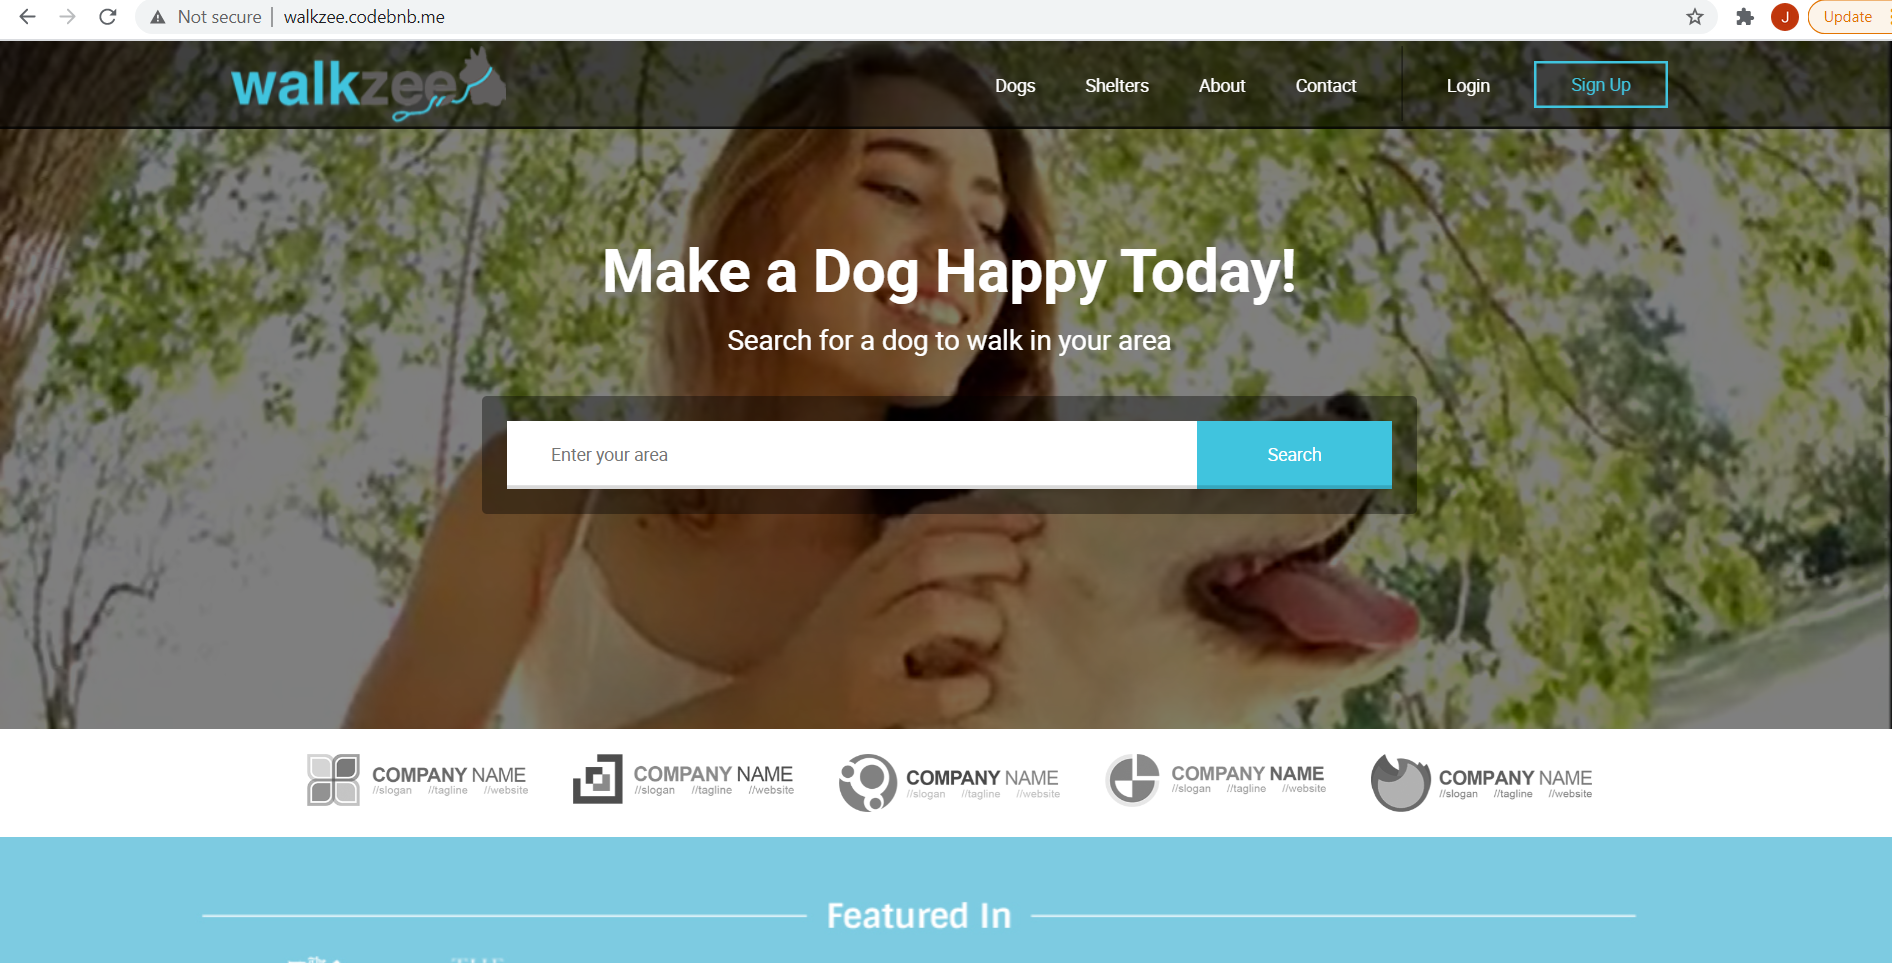
\includegraphics[scale=0.3]{slike/walkzee.png}
			\caption{Walkzee -- naslovna stranica}
			\label{fig:walkzee}
		\end{figure}

		
		\begin{figure}[htb]
			\centering
			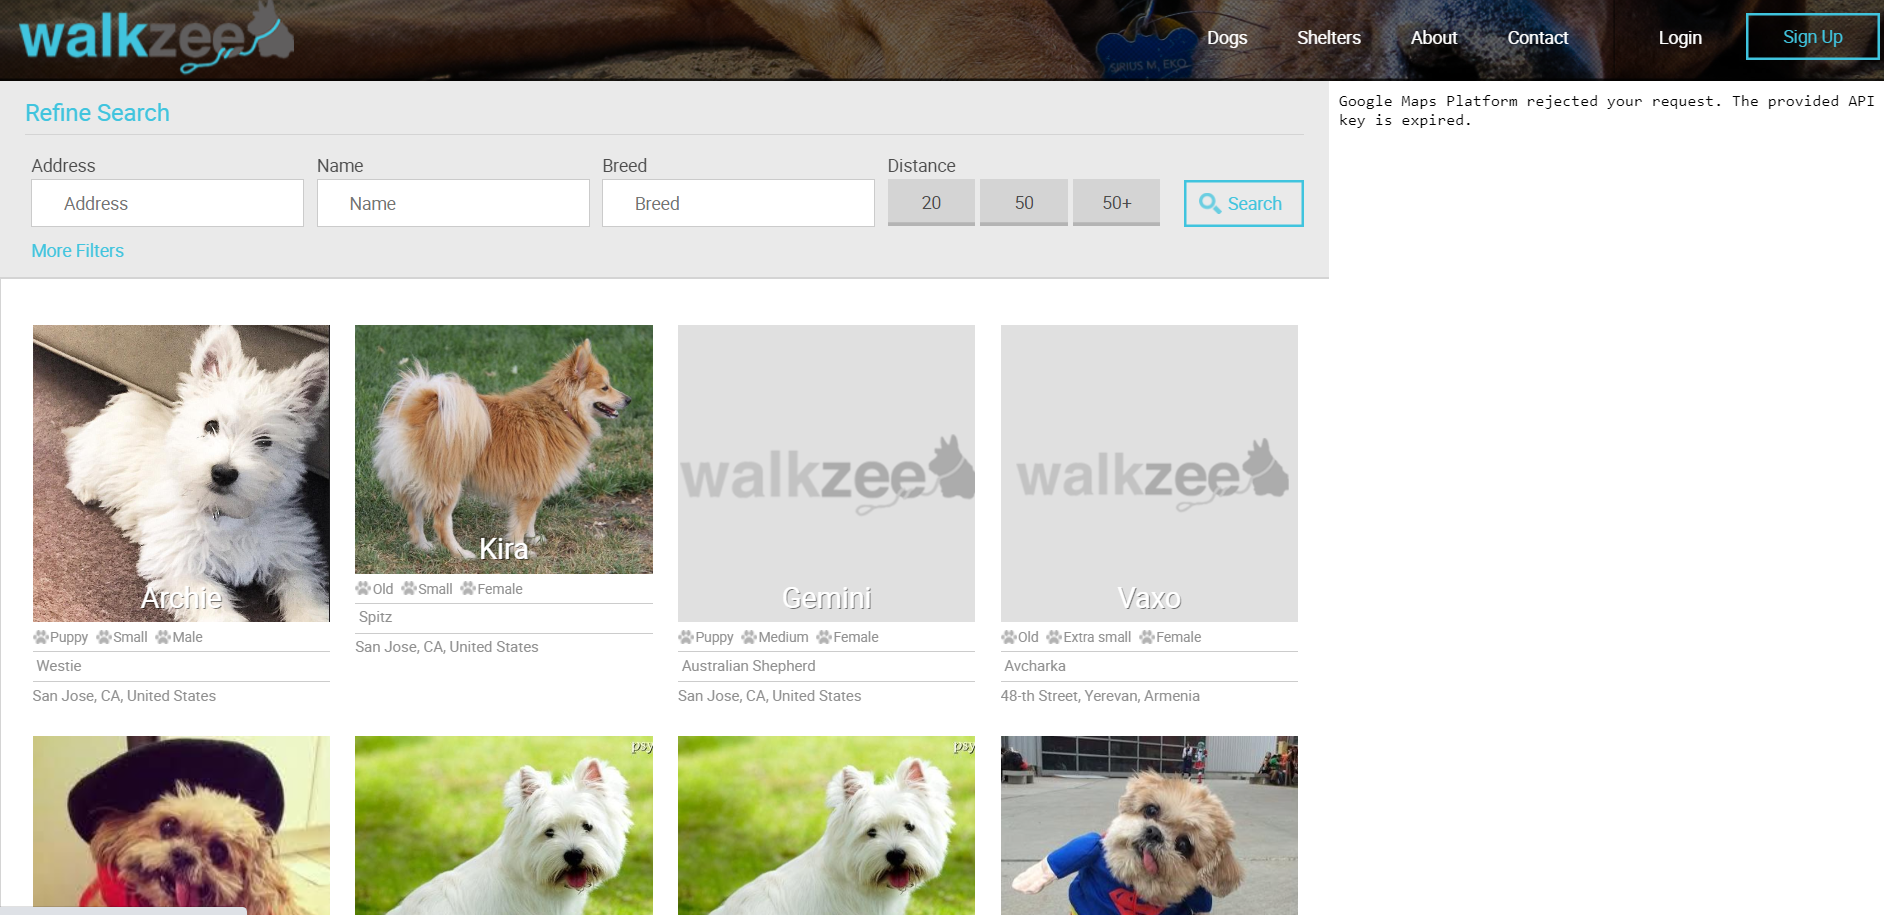
\includegraphics[scale=0.3]{slike/walkzeeDogs.png}
			\caption{Walkzee -- pregled pasa}
			\label{fig:walkzee}
		\end{figure}
	
	\section{Opseg projektnog zadatka}
	  \vspace{15pt}
		Glavni zadatak aplikacije je povezati udruge za životinje s građanima koji imaju
	želju i vrijeme za šetanje pasa, te time povećati izglede udomljavanja pasa i psihološkog
	efekta dobrobiti socijalizacije za psa i za čovjeka. \par \vspace{10pt}
	Aplikaciju će koristiti registrirane udruge za životinje, registrirani
	građani i javni posjetitelji koji nisu registrirani i imaju mogućnost
	pristupa naslovnoj stranici aplikacije i detaljima profila udruge.
	Udruge i građani se mogu registrirati, pri čemu građani upisuju sljedeće podatke:
	\begin{itemize}
		\item ime
		\item prezime
		\item korisničko ime
		\item adresa e-pošte
	\end{itemize} 
	a udruge još dodatno:
	\begin{itemize}
		\item naziv udruge
		\item OIB udruge
	\end{itemize}
	 \vspace{10pt}
	\underline{Javni posjetitelj} može doći u aplikaciju i
	pregledati sve udruge na naslovnoj stranici, zatim otići na detalje profila pojedine udruge,
	a osim toga ima i uvid u rang listu registriranih šetača.  Rang lista prikazuje poredak šetača
	s obzirom na broj šetnji, broj pasa, te duljinu šetnje koju su odradili u prethodnih mjesec
	dana.
	Na profilu pojedine udruge, posjetitelj može dobiti uvid u profile pasa,
	statistike o šetanjima svih pasa, lokaciju, te mogućnost prijave za šetanje pasa (ako se registrira). Statistika
	o šetnjama pruža informacije koji psi su češće bili u šetnji od ostalih, te time koji psi imaju
	veću potrebu za šetnjom.
	Ukoliko posjetitelj odluči pripomoći udruzi i priključiti se šetnji
	pasa, ima opciju registracije. Registracijom posjetitelj postaje registrirani građanin. 
	
	
	  \vspace{15pt} \par 
	  
	  	\underline{Registrirani građanin} ima opciju prijave u vlastiti profil i pregleda vlastitih rasporeda šetanja,
	  vlastitih statistika šetnji, zajedno s mogućnošću označavanja statistike šetanja kao javnih;
	  kako bi podaci građana dospjeli na rang listu na javnoj stranici.
	  Svi registrirani korisnici imaju mogućnost mijenjanja podataka u svom profilu.
	   Građanin može odabrati psa/e, odabrati željeni
	  termin šetnje i prijaviti se za šetača. Termin šetnje se odabire u obliku datuma i vremena.
	  Nakon uspješnog „rezerviranja“ psa za šetnju, termin za odabranog psa vidljiv je na
	  kalendaru registriranim građanima. Građani imaju opciju skinuti 
	  raspored za odabrani dan, tjedan ili mjesec u PDF obliku.\par
	  \vspace{15pt}
	
	Svaka \underline{registrirana udruga} može kreirati vlastiti profil koji će se prikazivati na javnoj
	stranici. Stranica udruge će sadržavati neke bitne detalje vezanu uz samu udrugu poput: 
	\begin{itemize}
		\item ime udruge
		\item voditelj udruge
		\item lokacija udruge
		\item kontakt: e-mail adresa
		\item OIB udruge
		\item IBAN udruge (za moguće donacije)
	\end{itemize}
Također, svaka udruga održava listu vlastitih pasa koji su raspoloživi za šetnju. Neke od bitnih informacija o pojedinom psu uključuju: 
	\begin{itemize}
		\item ime psa
		\item vrsta psa (ako je poznata)
		\item slika psa 
		\item opis psa (osobnost, izgled)
		\item dob psa
		\item raspored odnosno raspoloživost psa za određeni vremenski period (datum i vrijeme) 
		\item za kakve šetnje je pas predodređen (skupne ili individualne šetnje). 
	\end{itemize}
Svaka udruga ima opciju mijenjati svoj profil. To može uključivati mijenjanje vlastitih podataka (vezanih uz samu udrugu) te uređivanje liste i profila pasa. 




	  

		\iffalse
		\section{Primjeri u \LaTeX u}
		
		\textit{Ovo potpoglavlje izbrisati.}\\

		U nastavku se nalaze različiti primjeri kako koristiti osnovne funkcionalnosti \LaTeX a koje su potrebne za izradu dokumentacije. Za dodatnu pomoć obratiti se asistentu na projektu ili potražiti upute na sljedećim web sjedištima:
		\begin{itemize}
			\item Upute za izradu diplomskog rada u \LaTeX u - \url{https://www.fer.unizg.hr/_download/repository/LaTeX-upute.pdf}
			\item \LaTeX\ projekt - \url{https://www.latex-project.org/help/}
			\item StackExchange za Tex - \url{https://tex.stackexchange.com/}\\
		
		\end{itemize} 	


		
		\noindent \underbar{podcrtani tekst}, \textbf{podebljani tekst}, 	\textit{nagnuti tekst}\\
		\noindent \normalsize primjer \large primjer \Large primjer \LARGE {primjer} \huge {primjer} \Huge primjer \normalsize
				
		\begin{packed_item}
			
			\item  primjer
			\item  primjer
			\item  primjer
			\item[] \begin{packed_enum}
				\item primjer
				\item[] \begin{packed_enum}
					\item[1.a] primjer
					\item[b] primjer
				\end{packed_enum}
				\item primjer
			\end{packed_enum}
			
		\end{packed_item}
		
		\noindent primjer url-a: \url{https://www.fer.unizg.hr/predmet/proinz/projekt}
		
		\noindent posebni znakovi: \# \$ \% \& \{ \} \_ 
		$|$ $<$ $>$ 
		\^{} 
		\~{} 
		$\backslash$ 
		
		\begin{longtabu} to \textwidth {|X[8, l]|X[8, l]|X[16, l]|} %definicija širine tablice, širine stupaca i poravnanje
			
			%definicija naslova tablice
			\hline \multicolumn{3}{|c|}{\textbf{naslov unutar tablice}}	 \\[3pt] \hline
			\endfirsthead
			
			%definicija naslova tablice prilikom prijeloma
			\hline \multicolumn{3}{|c|}{\textbf{naslov unutar tablice}}	 \\[3pt] \hline
			\endhead
			
			\hline 
			\endlastfoot
			
			\rowcolor{LightGreen}IDKorisnik & INT	&  	Lorem ipsum dolor sit amet, consectetur adipiscing elit, sed do eiusmod  	\\ \hline
			korisnickoIme	& VARCHAR &   	\\ \hline 
			email & VARCHAR &   \\ \hline 
			ime & VARCHAR	&  		\\ \hline 
			\cellcolor{LightBlue} primjer	& VARCHAR &   	\\ \hline 
			
		\end{longtabu}
		

		\begin{table}[H]
			
			\begin{longtabu} to \textwidth {|X[8, l]|X[8, l]|X[16, l]|} 
				
				\hline 
				\endfirsthead
				
				\hline 
				\endhead
				
				\hline 
				\endlastfoot
				
				\rowcolor{LightGreen}IDKorisnik & INT	&  	Lorem ipsum dolor sit amet, consectetur adipiscing elit, sed do eiusmod  	\\ \hline
				korisnickoIme	& VARCHAR &   	\\ \hline 
				email & VARCHAR &   \\ \hline 
				ime & VARCHAR	&  		\\ \hline 
				\cellcolor{LightBlue} primjer	& VARCHAR &   	\\ \hline 
				
				
			\end{longtabu}
	
			\caption{\label{tab:referencatablica} Naslov ispod tablice.}
		\end{table}
		
		
		%unos slike
		\begin{figure}[H]
			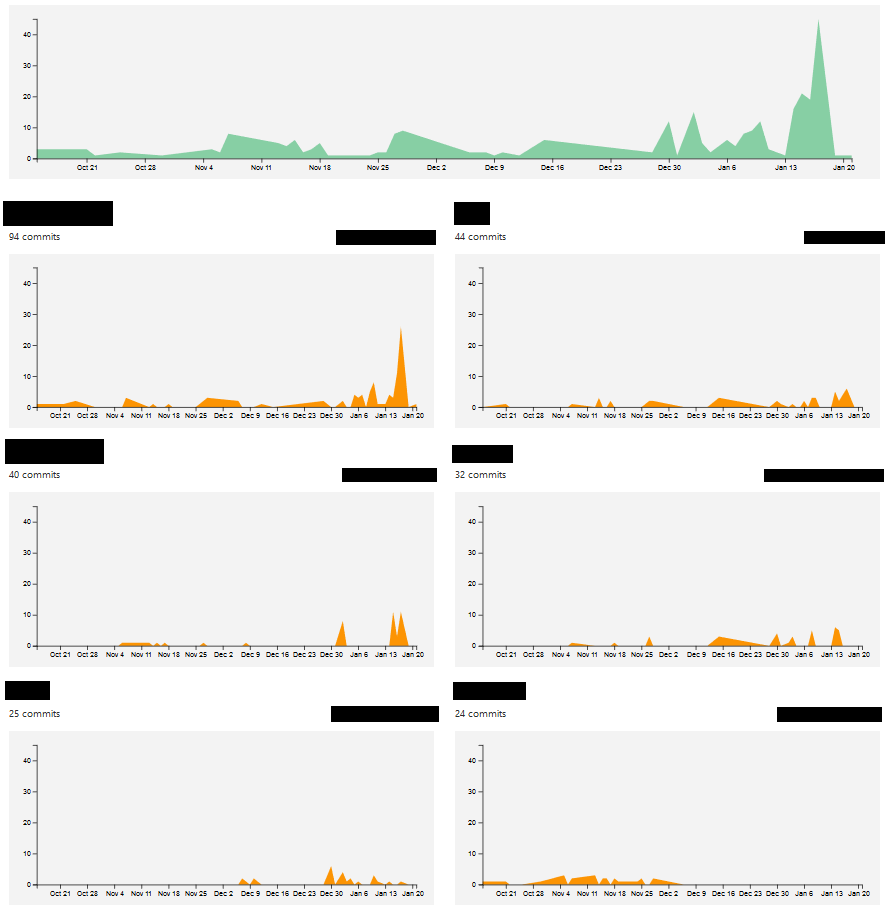
\includegraphics[scale=0.4]{slike/aktivnost.PNG} %veličina slike u odnosu na originalnu datoteku i pozicija slike
			\centering
			\caption{Primjer slike s potpisom}
			\label{fig:promjene}
		\end{figure}
		
		\begin{figure}[H]
			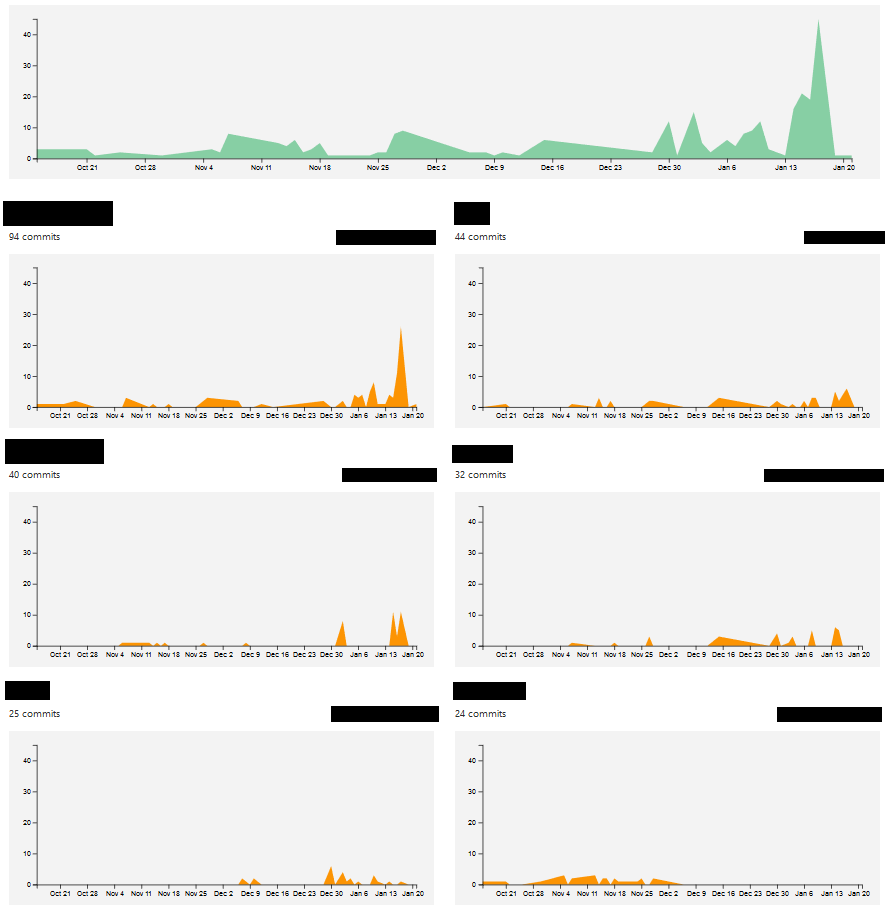
\includegraphics[width=.9\linewidth]{slike/aktivnost.PNG} %veličina u odnosu na širinu linije
			\caption{Primjer slike s potpisom 2}
			\label{fig:promjene2} %label mora biti drugaciji za svaku sliku
		\end{figure}
		
		Referenciranje slike \ref{fig:promjene2} u tekstu.
		
		
		\fi
		\eject
		
	